\documentclass[12pt, oneside]{extbook} % the document type needs to be change
\usepackage{geometry}
\usepackage{listings}
\usepackage{graphicx}

\geometry{
	a4paper,
	left = 1.5 cm,
	right = 1.5 cm,
	top = 2cm,
}

\title{Network and System Defense}

\begin{document}
\maketitle
\tableofcontents
\newpage
\part{Parte Hardware}
\chapter{Introduzione}
In cybersecurity, ci sono almeno 5 aree esterne differenti che si mischiano fra loro, e poi 3 aree interne relative all'hardware ed al software.\\ "L'attore principale" sono applicazioni Internet-based:
\begin{itemize}
\item vulnerabilità del sistema, della rete etc
\item come difendersi o evitare tali vulnerabilità, o almeno mitigarle
\end{itemize}
Molta configurazione pratica: laboratori da 0, ma è utile rifare tutto a casa (\textbf{CAZZI}).\\ Per via del fatto che è davvero difficile oggi separare cosa è la rete da cosa è il software, è utile parlare di tutti i diversi campi che riguardano sia la rete che il software.\\ Punti chiave:
\begin{itemize}
\item Access networks and perimetral security: Ethernet, VLAN, IPv6, 802.11x, firewall, packet classification algorithms
\item Core networks: BGP, MPLS, DDos e Botnets, VPNs con BGP
\item End to End security: PKIs, DNS security, HTTPS, Overlay VPNs
\item Sw and Operating System
\item Virtualization \& Cloud 
\end{itemize}
Piattaforme da utilizzare per la parte da 6 CFU (Hardware):
\begin{itemize}
\item GNS3
\item Tinycore Linux
\item VMware o Virtual Box: Virtual Box sembra lavorare meglio con GNS3
\item Cumulus Linux: serve per emulare le funzionalità di livello 2 di uno switch. Net OS, \textbf{scaricare la versione 4.1} e non le ultime. C'è un insieme di VM pronte per essere installate su un virtualizzatore
\item Immagini CISCO (da cercare online, if you know what I mean)
\item Lubuntu
\item Ubuntu server
\end{itemize}
\chapter{Introduzione alla cybersecurity}
Ci sono 3 fattori principali quando si parla di cyberscurity:
\begin{itemize}
\item Cosa bisogna proteggere?
\item Da quali minacce? Ci sono diverse fonti di attacco da cui proteggersi
\item Come fare per contrastare queste minacce? Integrità, encryption, etc...
\end{itemize}
\paragraph{Definizione di computer security:}le misure ed i controlli che garantiscono confidenzialità, integrità e disponibilità degli assets dei sistemi informativi, incluso hardware, software etc...
\begin{itemize}
\item confidenzialità: i dati sono privati, le informazioni confidenziali non sono note ad entità non autorizzate. Esempi: usare SSH o HTTPS per scambiare credenziali con un server.
\item Privacy: (slides)
\item Integrità: se dei dati, indica che essi sono cambiati solo in maniera autorizzata. Se voglio traferire un messaggio con cui trasferisco del denaro, non voglio che il contenuto sia compromesso. Se si parla di integrità dei sistemi, si intende che il sistema performi come deve (vedi slides)
\item disponibilità: si assicura che il sistema lavori in maniera corretta e che i servizi non siano negati ad utenti autorizzati
\end{itemize}
Altri aspetti importanti:
\begin{itemize}
\item Authenticity: dell'utente, indica che sia possibile verificare che l'utente è chi dice di essere. Della sorgente: capacità di verificare che un messaggio arriva da una sorgente effettivamente affidabile.
\item altri ... (slides)
\end{itemize} 
\textbf{ALTRE IMPORTANTI DEFINIZIONI CHE SI TROVANO SULLE SLIDES}. \\ Quali sono le diverse superfici di attacco:
\begin{enumerate}
\item la rete stessa: i sistemi sono Internet-based, quindi è sempre possibile attaccare la rete. Attaccare la rete implica sfruttare vulnerabilità della rete Internet: ARP, WEP, link fisici, intrusioni nella rete etc...
\item attacchi al software: vulnerabilità nell OS, server web, code injection etc...
\item attacchi all'umano: molte vulnerabilità create da noi stessi, social engineering, errori umani, mancanza di competenze etc...
\end{enumerate}
È importante non pensare che la sicurezza sia data solo dalla tecnologia, ma anche dalle persone.\\ \paragraph{CIS critical security controls:} 20 applicazioni pratiche che la SANS suggerisce di applicare per verificare la sicurezza di una corporation (anche piccola Enterprise). Ogni controllo ha dei sotto-controlli più "concreti"\\ Quindi, non avendo il tempo di fare tutto, ci concentrare su alcuni aspetti fondamentali di tutto l'insieme visto.
\section{Lezione 2: vulnerabilità intrinseche IP/TCP}
Prima di capire le vulnerabilità, è necessaria una revisione dei protocolli di rete.
\subsection{Architettura di IP}
Intenet non è altro che una inter-connessione di reti che possono avere differenti tecnologie.\\ La comunicazione fra i device è possibile con IP, che è implementato sui livelli 1 e 2 (che sono indipendenti). Ogni dispositivo è identificato dall'indirizzo univoco a 32/64 bit (che seguono la nomenclatura CIDR), le diverse sotto-reti comunicano tramite i router ovvero un device IP che ha almeno 3 livelli dello stack Internet. Ha diverse interfacce che possono essere in diverse tecnologie: ADSL, Ethernet, Fibra etc...\\ Le operazioni compiute dai router:
\begin{itemize}
\item IP forwarding: longest prefix mathcing, manda un pacchetto verso la prossima interfaccia del percorso di rete. È diretta se la destinazione è nella subnet, mentre indiretta se serve trovare il next hop, quindi andare fuori dalla propria sotto-rete. Il next hop è un dispositivo nella propria sotto-rete che sa come arrivare alla destinazione.
\end{itemize}
Il goal di IP è quello di mandare il pacchetto a destinazione, l'Internet è diviso in Autonomous Systems all'interno dei quali si può configurare il routing come si vuole. Ma poi, serve scambiare informazioni fra As, si parla quindi di protocolli intra-AS come OSPF, RIP e protocolli inter-AS, come BGP.\\ C'è l'header per ogni pacchetto che ha i diversi campi (TTL, src, dest, protocol, checksum etc...), diverso fra IPv4 ed IPv6, differenze fra i due:
\begin{itemize}
\item header più piccolo in IPv6
\item no fragmentation in IPv6
\end{itemize}
\paragraph{Routing table:}struttura dati che associa una destinazione ad un next hop. Per il routing si usa il longest prefix matching, l'IP più "specifico" è quello scelto. La differenza principale fra host e router è che se un host riceve un pacchetto da una src non fra quelle locali, lo scarta; un router lo forwarda. Il forwarding standard basico è fatto in base all'indirizzo di destinazione. Dopo l'estrazione del pacchetto IP, se l'IP dest è locale, lo manda al livello superiore, altrimenti lo guarda nella tabella di routing: se non si trova un matching, il pacchetto è scartato. Altrimenti: se c'è un next hop, bisogna scoprire chi è, altrimenti basta scoprire il MAC associato all'IP.\\ La maggior parte dei pacchetti che vengono mandati vanno fuori dall'AS con cui si firma il contratto: possono esserci diversi AS di transito prima di arrivare al data center del sito a cui si cerca di connettersi.
\subsection{Vulnerabilità di TCP/IP}
Per design, IP e TCP non si preoccupano della sicurezza in quanto sono stati progettati quando la sicurezza non era un problema. C'è un certo numero di vulnerabilità intrinseche nei protocolli, ed è ancora così in quanto sono stati progettati senza pensare all'aspetto di sicurezza:
\begin{itemize}
\item Identification: i device della rete possono essere falsificati, è possibile spoofare l'IP address per dire di essere , ad esempio, un certo server web. Sia per i pacchetti generati dall'utente che per quelli forwardati. Se mandiamo un pacchetto di un legittimo server DNS, stiamo impersonificando il server stesso. Non ci sono meccanismi in IP per verificare l'autenticità di chi manda il pacchetto
\item Reputation: come è possibile verificare che l'origine del pacchetto è effettivamente la sorgente?
\item Confidentiality: non vogliamo che le informazioni scambiate sulla rete siano viste da 3e parti. Vorrei che solo il server veda i dati in uno scambio client-server. Ma intercettare il pacchetto in maniera "malevola" è fattibile ed anche decodificarlo perché l'header e l'IP sono in chiaro.\\ Il problema non è nella rete interna, ma passa per diversi AS (noi ci fidiamo solo del nostro): anche se il path fra sorgente e destinazione è fidato, è possibile fare hijaking su BGP, fra gli attacchi più pericolosi e in voga.
\item Integrity: voglio essere sicuro che il pacchetto non sia modificato durante il percorso fra src e dest. C'è il checksum, ma è calcolato su dati in chiaro, quindi non va bene come "codice" per poter assicurare l'integrità
\item Packet replication: non c'è sequence number nell'IP header nella sessione, non ci sono meccanismi per proteggersi da questo threat
\end{itemize}
\subsubsection{Dynamic mapping}
Le cose si complicano perché i protocolli Internet usano diversi meccanismi per implementare il mapping: ad esempio il DSN, ARP, 802.3 bridging (lo switch impara in automatico quale MAC è dietro quale porta) e questo è dinamico in quanto può cambiare nel tempo. Questo problema è presente in ogni layer ed anche questi meccanismi non sono stati penasti per essere sicuri.
\paragraph{DNS spoofing:}possiamo spoofare una richiesta DNS, quindi fare un hijack della sessione. Attacco triviale (e vecchio):
\begin{itemize}
\item sfruttiamo il mapping MAC-IP per diventare MiTM
\item sfruttiamo il mapping fra il nome di dominio e l'IP per impersonare il server web
\item mappiamo l'IP del sito al nostro
\end{itemize}
Lo scenario è che l'attaccante sia nella stessa sotto-rete.\\ L'idea è quella di mandare dei messaggi ARP spoofati per far credere alla vittima di essere il default gateway e di fra credere al default gateway di essere la vittima.\\ Per impersonare il sito target è possibile usare il comando \textsf{wget}, ed usare Apache2 per impersonare il server web.\\ L'attacco sfrutta 3 vulnerabilità:
\begin{itemize}
\item ARP spoofing
\item DNS redirection
\item Impersonification
\end{itemize}
Per emulare un server DNS è possibile configurare bind ma c'è un piccolo servizio DNS da configurare e che permette di forwardare all'attacker tutto ciò che sono è noto.
\subsection{Security requirements per le vulnerabilità}
Vediamo cosa è possibile risolvere questi problemi: per la confidenzialità si usano algoritmi a chiave simmetrica per garantirla.\\ Un algoritmo a chiave simmetrica, entrambe le end della comunicazione condividono la stessa chiave, c'è anche la differenza fra:
\begin{itemize}
\item stream ciphers 
\item block ciphers, che usano concatenazione per evitare ECB, in cui se la stessa chiave viene riusata per molto è possibile scoprire il contenuto di blocchi che hanno lo stesso contenuto
\end{itemize}
Per l'integrità, vogliamo una prova che nessuno modifichi il contenuto del messaggio, quindi si produce un MAC basato su hash functions: l'hash è calcolato non solo sui dati ma anche sulla chiave.\\ L'Authenticated Encryption permette, con "la stessa chiave" di fornire sia confidenzialità che integrità. Si può ottenere un algoritmo del genere anche con le tecniche base di symmetric encyption.\\ Per l'autenticità è possibile usare pub key cryptography per realizzare dei meccanismi di firma, come RSA e Diffie-Hellman. Serve comunque avere una certificazione che un utente è il vero proprietario di una chiave, quindi che sia crittograficamente legato alla chiave: Public Key Infrastructure.
\section{Lezione 3: Ethernet LAN security}
Ethernet è una tecnologia di livello 2, il primo standard open e multi-vendor nato nel 1976.\\ L'802 è una famiglia di standard dell'IEEE, fra di essi ci sono diversi gruppi di lavoro e quello che si occupa di Ethernet è 802.3 e quindi si parla di questi standard, in quanto Ethernet era il nome commerciale.\\ La trama Ethernet originale ha un header molto snello, c'è il campo type / length che può essere due campi differenti a seconda della situazione (vedi slides)\\ Anche in questo caso è tutto in chiaro, quindi ci sono gli stessi problemi. Gli indirizzi MAC sono a 48 bit
\paragraph{Hub, Switch e Bridge:} un hub è uno strumento che forwarda pacchetti verso tutti. Uno switch ha un forwading database, ovvero una struttura dati che associa MAC alle porte. Lo switch impara in automatico quale è il MAC dietro una certa porta. Il problema sta proprio nel fatto che lo switch impara in automatico il mapping.\\ Si usa l'algoritmo spanning three per evitare i loop, che si possono creare perché, per motivi di ridondanza, è possibile avere dei loop nella rete.\\\\ Per operare al di sopra di Ethernet, IPv4 usa ARP e DHCP mentre IPv6 usa NDP, protocollo simile. NDP non è sicuro, ma c'è un protocollo per renderlo sicuro e lo stesso protocollo è stato progettato già pensando alla sicurezza.\\ Anche nel caso di DHCP, usato per ottenere un IP, abbiamo gli stessi problemi detti sopra.
\subsection{Ethernet LAN vulnerabilities}
Quali sono le possibili contro-misure per difendersi dai threats. I problemi di Ethernet sono dovuti al fatto che per natura si auto.configura. Siccome è possibile avere accesso a qualunque trama Ethernet, l'attaccante può:
\begin{itemize}
\item imparare qualcosa sulla topologia della rete
\item avere accesso agli switch
\item eavesdropping
\item etc...
\end{itemize}
Vediamo alcune categorie di problemi
\subsubsection{Network and system access}
Come è possibile ottenere accesso ad un Ethernet segment: unioni non autorizzate:
\begin{itemize}
\item tramite accesso fisico allo switch, se la porta è attiva
\item accedere ad una socket a muro
\item rimuovere il cavo ad un PC e metterlo in un altro
\item inserire uno switch fra il PC esistente e la socket
\end{itemize}
Espansioni della rete non autorizzate.\\ Un altro modo per ottenere l'accesso è quello di accedere in maniera remota, o anche fare il probe della rete per scoprire informazioni, come ad esempio usare nmap. Altri modi:
\begin{itemize}
\item break-ins
\item switch control: uno switch che ha password di default o non la ha e la password può essere resettata fisicamente. Se si ottiene il controllo di uno switch si possono fare varie cose, ad esempio se lo switch gira su cumulus Linux
\end{itemize}
Una volta che si è ottenuto l'accesso alla rete, si può fare lo sniffing del traffico di rete. Oggi non è più vero che la trama arriva a tutti e che sono tutti connessi, se la possibilità di intercettare fisicamente il pacchetto, è possibile fare un MiTM etc...\\ Ma il problema è anche nella procedura di learning dello switch: il MAC non è autenticato, quindi mandando una trama con un MAC reale allo swtich, viene ingannato nel pensare che il MAC è dietro una porta sbagliata.\\ Quindi l'attaccante può redirigere il traffico trasmesso dalla vittima verso se stesso, anche se è più che altro teorico perché anche la vittima manda messaggi.\\ Si può generare un pacchetto con un indirizzo falso, o anche intercettare un pacchetto e cambiarlo in quanto anche a livello 2 non c'è integrity check o HMAC tag.\\ Per cambiare il MAC, ci sono vari modi:
\begin{itemize}
\item cambiare il MAC della NIC (comando Linux)
\item usare raw socket programming
\item in-kernel programming
\end{itemize}
Per intercettare il pacchetto, basta mettere l'interfaccia di rete in modalità promiscua per ricevere tutto il traffico anche non diretto a me, così da poter cambiare il MAC.
\paragraph{MAC flooding:}l'idea è di inondare lo switch con un grande numero di trame con diversi indirizzi MAC per saturare la memoria dello switch in modo da far si che tutti i pacchetti siano inviati verso tutte le porte in broadcast.\\
\paragraph{ARP e DHCP poisoning:}si può fare ARP poisoning (vedi sopra) ma anche facendo poisoning di DHCP facendo creder di essere il server, spoofando tutto lo scambio DHCP.\\ Nell'ARP poisoning si avvelena tutta la ARP cache, che è usata per memorizzare risultati di precedenti ARP request per evitare di rifarle ogni volta (ogni riga ha comunque un TTL). È sempre possibile configurare la cache ARP in maniera statica. Le ARP gratuite sono utili per vari motivi, non solo pericolosi. È possibile fare un MiTM: ho un PC ed un default gateway, mando una ARP response (op code 2) col MAC della vittima al default gateway ed una ARP response col MAC del default gateway alla vittima.\\ (N.B:ARP non è stato progettato specificamente per mappare IP-MAC, ma per associare un indirizzo di layer 3 ad uno di layer 2).
\paragraph{Session hijack: }a livello 2, Ethernet non ha conoscenza della sessione, è come IP: non c'è relazione fra pacchetti inviati in sequenza, e questo è un'altra vulnerabilità. È possibile dirottare una sessione e iniziare a trasmetterli in una sessione già stabilita, perché Ethernet non ha protezioni per questo.
\paragraph{Denial of service:}l'obiettivo è quello di negare il servizio, si può fare nel layer Ethernet. È possibile esaurire le risorse di una macchina, cercare di far crashare lo switch ma anche farlo a livello di protocollo. STP (Spannign Three)permette di gestire grandi topologie di rete, con molti switch e link ridondanti, quindi loop fisici. Con STP si disabilita la porta che causa il loop, ma anche STP non  autenticato e si può far credere di essere uno switch.
\subsection{Contromisure}
Per risolvere i problemi, è stato deciso che tutte le trame Ethernet vengano marcate come non sicure. Per farlo è necessario metterlo in un dominio protetto, ovvero protezioni perimetrali come il firewall etc... Altrimenti, è possibile usare soluzioni crittografiche, in ogni caso ci sono 4 categorie di contromisure:
\begin{itemize}
\item router based security: se si può rimpiazzare uno switch con un router, si risolvono molti problemi. Un IP router messo fra tutti i nodi, non c'è un singolo dominio di broadcast, che è interrotto perché il router non forwarda i pacchetti in broadcast. In questo modo si risolvono ARP, STP, MAC table based attacks. (Si possono avere dei singoli dominii di broadcast usando le VLAN.)
\item access control: se non si può sostituire con un router, si può comunque controllare chi accede alla rete in differenti modi. Per farlo, uno dei modi è usare il protocollo 802.1X port authentication: l'idea è che la porta di uno switch è aperta solo se il client s è autenticato correttamente verso un'altra entità, che è l'authentication server. Un altro modo è usare le ACL (Access Control List), (RIFAI IL LABORATORIO 2)\\ Il problema rimane, perché i MAC sono comunque spoofabili e quindi i pacchetti non sono comunque protetti e possono essere forgiati a piacere
\end{itemize}
\subsubsection{Central managed LAN}
Sarebbe utile avere una entità centrale per poter garantire l'accesso in rete ed i progetti sono per lo più di ricerca:
\begin{itemize}
\item SANE: ogni client ha del software e prima di poter comunicare con lo switch deve mandare una richiesta al punto centrale
\item Ethane: i client non devono avere nessun software sull' IP/TCP stack: per ogni pacchetto, è lo switch a mandare i pacchetti alla entità centrale ed è quella che dice se i pacchetti vengono accettati oppure droppati.\\ È simile al concetto dell SDN: il controllo è separato dai dati, il data plane è staccato dal control plane. L'idea è che il software procede molto più velocemente dei protocolli di rete, perché è più facile e ci sono interfacce di programmazione ben definite. Non è facile invece aggiornare un protocollo e come questo viene implementato: l'hardware è comunque più veloce del software in quanto è specializzato mentre per il software c'è un grande overhead dovuto al SO, al kernel etc... mentre l'hardware è dedicato.
\paragraph{OpenFlow} una delle prime implementazioni di SDN, lo stack di networking è diviso in data plane e control plane. OpenFlow definisce come è fatto il data plane ed anche il protocollo per iniettare il codice di configurazione nel control flow. Inoltre, OpenFlow è fatto da una pipeline di flow table, per cui se ho un miss nella tabella di routing il controllo passa al control plane che è fatto nel linguaggio preferito. Quindi, dopo averlo processato, viene rimandato allo switch con un comando (regola) che dice come trattare tutti i successivi pacchetti dallo stesso IP.\\ Non è stata progettata per essere sicura ma il processamento: una volta che ho imparato dal primo pacchetto cosa fare, tutti gli altri sono processati velocemente. Non è scalabile, in quanto il control plane centralizzato riceve tutti i pacchetti nuovi e diventa il collo di bottiglia. Viene però centralizzata la decisione su cosa fare per i pacchetti, come dicevamo sopra.
\end{itemize}
\subsubsection{Sicurezza dei protocolli: MACsec}
Perché non applicare un approccio crittografico per la sicurezza al livello 2: abbiamo TLS ed IPSec per il 5 ed il 3. Abbiamo MACsec, che è come l'IPsec per Ethernet. Definisco il parametro dell'associazione, non sono obbligatori, ma abbiamo
\begin{itemize}
\item confidenzialità
\item integrità
\item anti-replay
\end{itemize}
È più simile ad IPsec, in quanto TLS è all-in-one: definisce sia come implemetare le sessioni sicure che come fare l'handshake. Mentre MACsec non definisce la fase di negoziazione, che è fatta con un protcollo apposito.\\ L'header di MACsec può avere come opzionali il TAG per l'autenticazione e la parte di encryption. Serve anche il sequence number perché Ethernet non è reliable, a differenza di TLS che poggia su TCP. Come in IPsec, la Security Association che viene creata è mono-direzionale e quindi va ogni volta creata in entrambe i versi della comunicazione.
\subsubsection{Security monitoring}
Ci può essere controllo sull'accesso alla rete, ma non si può essere sicuri che i client non siano malevoli. Si può quindi monitorare il traffico con un Ethernet firewall ma non ha senso fare la differenza dei firewall ai diversi livelli.\\ Altrimenti ci sono IDS e Prevention System, le implementazioni più importanti open source sono (slides)
\subsection{IPv6 neighbour discovery}
La prima motivazione per implementare IPv6 è che l'IPv4 ha indirizzi troppo corti che sono finiti, ma le altre motivazioni riguardano il neighbour discovery. In IPv4 ci sono vari protocolli come DHCP, ICMP, ARP che sono di controllo e gestione, in IPv6 è tutto unificato e fatto da ICMPv6 in maniera migliore e più chiara.\\ La neighbour discovery viene fatta per capire il MAC associato ad un IPv6, o chi è il deafult gateway etc... e può essere fatto tutto con IPv6 neighbour discovery; non è un meccanismo in se ma un protocollo che definisce dei messaggi, con cui si può
\begin{itemize}
\item scoprire un gateway
\item fare redirection
\item etc...
\end{itemize}
I messaggi base definiti da ICMPv6 per il protocollo di neighbour discovery sono i seguenti
\begin{itemize}
\item Router Solicitation
\item Router Advertisment
\item slides 
\end{itemize}
Ogni combinazione di messaggi viene usata per fare una delle azioni che in IPv4 viene fatta con un protocollo apposito
\subsubsection{Neighbour solicitation e Advertisment}
In questo caso, un nodo può usare degli indirizzi speciali:
\begin{itemize}
\item multicast verso tutti: indirizzo con prefisso (FF02::1, destinazione) (:: = 0:0...)
\item Multicast verso tutti i router: (FFO2::1, dest)
\item indirizzo multicast per fare solicitation
\end{itemize}
Per fare Address Resolution si manda il neighbour solicitation e si riceve il messaggio di risposta per poter risolvere il MAC associato ad un IPv6.\\ Anche in questo caso, non ci sono concetti di sicurezza 
\begin{itemize}
\item DoS: per configurare un IPv6 è possibile fare una cosa nuova, ovvero senza DHCPv6 perché la neighbour discovery è possibile scoprire chi sono i router, capire il prefisso della rete e serve solo la parte host dell'indirizzo. Siccome gli indirizzi sono molto lunghi, è possibile auto-configurare un IP che non collida con quello di qualche altro nodo della rete.\\ Ora, bisogna cercare se c'è duplicazione dell'IPv6. Se si vuole fare DoS, si intercettano i messaggi di richiesta duplicati e si dice che l'host esiste già.
\end{itemize}
ma la crittografia è implementata come estensione al protocollo con la Secure Neighbour Discovery: si usano 4 nuovi messaggi
\begin{itemize}
\item CGA: possiamo fare il binding fra IP address con un dispositivo senza una CA? Sì, un IP generato crittograficamente: abbiamo una chiave pubblica, ogni volta che mandiamo un messaggio lo firmiamo con la chiave privata e chiunque riceve può verificare che nessuno  sta spoofando quell'IP. I 64 bit più signifcativi sono il prefisso della rete e i restanti di host, ha anche dei parametri di sicurezza per pararsi da bruteforce attacks. La struttura dati associata alla CGA è la seguente: (slides)\\ La generazione avviene a partire dalla struttura dati della CGA: l'algoritmo scegli un modificatore random, seleziona un valore sicuro e mette il collision number a 0. Si fa SHA-1 e si prendono 112 bit, si verifica poi che 16*(sec leftmost Hash2 bits) sia 0, per poter essere robusti a bruteforcing. Se il prodotto non fa 0, si riparte e se dopo la generazione del CGA c'è una collisione, ovvero un IP duplicato va incrementato il counter della collision.\\ Siccome non è spiegato come controllarlo ma va fatto, ci sono vulnerabilità associate e quindi il controllo va protetto. Si continua poi con la generazione
%immagine di come continua
\\ La cosa importante è che c'è una chiave pubblica legata ad un IP address, in modo ad non avere una CA per ogni nodo che entra in una rete e quindi non sia richiesto un certificato.\\ È vero che si può generare una CGA propria se si è un attaccante, ma le CGA non sono usate per fare authorization, quindi non è possibile spoofare un address perché dovrebbe trovare una collisione nell hash function (che è crittografica) ed inoltre non si può generare la chiave privata associata alla chiave pubblica. Per questo, ci sono dei tipi di attacco differenti.\\ C'è una opzione della CGA per verificare la firma dopo aver verificato la CGA: se uno dei due controlli fallisce, il pacchetto non è valido
\item RSA signature: opzionale, metto una firma fatta con RSA nel messaggio. Se è un router, abbiamo la chiave pubblica del router, altrimenti quella pubblica del client associata all'IP
\item Nonce e Timestamp
\end{itemize}
col protocollo possiamo dimostrare (slides)
\paragraph{Router Authorization}
Otteniamo un messaggio di Router ? che è autenticato dal fatto che il router ha un certificato dato da una CA, se l'host ha la chiave della CA può verificare che il messaggio è effettivamente autentico.\\\\
\\ Mettendo tutto insieme, ICMPv6:
\begin{enumerate}
\item il nodo 1 vuole scoprire un certo MAC e quindi manda un messaggio di sollecitazione. Avrà una sua chiave pubblica (slides)
\item dopo tutto il pippone di roba, si firma tutto il pacchetto con la chiave privata usando l'agoritmo e si appende l'opzione della firma RSA e viene mandato il pacchetto
\end{enumerate}
Il receiver:
\begin{enumerate}
\item controlla la src
\item (slides)
\end{enumerate}
Si procede con i passi scritti sulle slides\\ Le conclusioni (slides)
\newpage
\part{Parte software}
\chapter{Introduzione}
Approccio bottom up a partire dall'hardware fino al software. Imparare i componenti interni di ogni livello dello stack prima di imparare l'attacco, in modo da capire meglio come funzionano. A questo punto, capire come e se è possibile incrementare il livello di sicurezza. Perché non dire che renderemo il sistema sicuro? È impossibile rendere un sistema sicuro, \textbf{un computer sicuro è scollegato dalla rete, con l'hw che prende fuoco.}
Argomenti che vedremo:
\begin{itemize}
\item attacchi hardware-based e contromisure
\item OS e principi di sicurezza
\item virtualizzazione
\item malware detection
\item DB security
\end{itemize}
\chapter{Hardware based attacks e contromisure}
Perché sono interessanti gli attacchi all'hardware: perché ogni sistema IT si basa sull'hardware, quindi compromettendo questo si riesce a compromettere tutto lo stack IT. Quando scrivo sw, mi aspetto qualcosa dall'hw e quindi se lo altero per il software è molto difficile capire che è compromesso.\\ I blocchi fondamentali per costruire degli attacchi hw based di successo:
\begin{itemize}
\item leggere primitive, per circumnavigare la sicurezza del sw
\item scrivere primitive
\item covertness: se l'attaccante può fare un attacco che non può essere scoperto è impossibile per il sw capire che c'è un attacco in corso
\end{itemize}
La prima cosa da fare è capire come funziona l'hw
\section{Storia dell'hw}
Legge di Moore: il numero di transistor di un calcolatore raddoppia di ogni anno.\\ Quindi possiamo aggiungere sempre più componenti nel chip: tempo fa si aveva il sw, si cambiava la frequenza del processore e il sw andava più veloce. Ma c'è un upper bound nella potenza consumabile, che è 130W e quindi anche aggiungendo componenti non si può sfruttare più potenza. Non si può aumentare la frequenza oltre il power wall, l'ammontare della potenza nel calcolatore è talmente alta che non si può aumentare la velocità della CPU.\\ Le CPU inizialmente erano multi ciclo e single core, già complesse ma lente. Quindi la prima cosa fu quella ci cercare di rendere più veloci:
\begin{enumerate}
\item la prima cosa fatta negli 80' fu l'introduzione del pipelining: allo stesso tempo, in parallelo, vengono processare diverse istruzioni che sono in diversi stadi della pipeline.\\ Si può committare una istruzione per ogni ciclo, ma si velocizza l'esecuzione delle istruzioni. Quindi la frequenza della CPU venne aumentata, ma si può sempre committare una istruzione alla volta
\item architettura super-scalare, aggiunge la possibilità di committare più istruzioni perché gli elementi base come alu, più elementi per il fetch etc... sono ridondati. Quindi, c'è l'istruzione nella pipeline e serve della logica nella CPU che dica quale hardware è disponibile e può essere assegnato alle istruzioni ogni volta, quindi serve un run-time scheduling. In ogni caso, ci sono i problemi della pipeline come i branch condizonali e la neceesità di dati quando non ancora disponibili
\item dai problemi sopra, nasce la speculazione:
\begin{lstlisting}[mathescape=true]
a $\rightarrow$ b + c
if a $\geq$ 0 then
	d $\leftarrow$ b
else
	d $\leftarrow$ c
\end{lstlisting}
fetcho un'istruzione prima di avere conoscenza del fatto che devo fare un salto piuttosto che un altro. Quindi ci sono una serie di bolle necessarie anche per un codice semplice, c'è una penalità per gli stalli enorme ed il codice fa molti salti.\\ Quindi, serve cambiare le cose: branch prediction. 
\end{enumerate}
\section{Branch prediction}
Se la predizione è sbagliata, si scarta il risultato, quindi si flusha una serie di stadi della pipeline perché incorretti, altrimenti si continua con l'esecuzione delle istruzioni. Ci sono delle parti dedicate nel chip del processore apposite per il branch prediction, migliore sarà la predizione e meno stalli si osserveranno e quindi migliori prestazioni. Le performance dipendono da due fattori: quanto presto si può controllare se la predizione è corretta e se la predizione è corretta.\\ Ci sono due tipi di predizione:
\begin{itemize}
\item \textbf{dynamic prediction}: implementata in hw, la predizione cambia in base al comportamento del sw. Basata tipicamente sulla storia dei branch
\item \textbf{static branch prediction}: determinata a compile time, come ad esempio il \textsf{likely} nel codice del kernel. Viene riflessa a livello assembly con dei prefissi come ad esempio \textsf{0x2e} o \textsf{0x3e} ma nelle architetture moderne non funziona più perché la pipeline è troppo complessa.
\end{itemize}
La branch prediction table è una piccola memoria nella CPU utilizzabile per capire l'outcome di una branch instruction: si usano i bit meno significativi dell'istruzione per indicizzare la tabella e prendere la decisione, il risultato è binario (take or not take). \\ Se la predizione è corretta ed è take ho un ciclo di penalità: questo perché si esegue l'istruzione di salto, ma nella pipeline c'è comunque la fase di fetch per cui semplicemente la carico, ma per poter fare la predizione devo arrivare almeno alla fase di decode.\\ Se la predizione è not take ed è corretta non ho penalità\\ Se invece la predizione è incorretta, devo 
\begin{itemize}
\item cambiare la predizione
\item aggiornare la tabella
\item flushare la pipeline, la penalità è la stessa che si avrebbe se non ci fosse la branch prediction, perché ci sarebbero gli stalli.
\end{itemize}
L'automa a stati che rappresenta i cambi di stato in base alla predizione è il seguente:\\\\
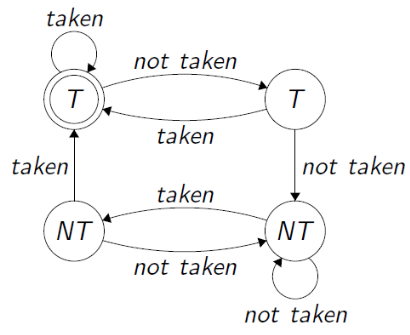
\includegraphics[scale=0.7]{immagini/2bit_pred}\\\\
si possono usare due bit per decidere come spostarsi in base alla predizione. Come si comporta con dei cicli annidati? 
\begin{lstlisting}
	mov $0, %ecx
.outerLoop:
	cmp $10, %ecx
	je .done
	mov $0, %ebx
.innerLoop:
	; actual code
	inc %ebx
	cmp $10, %ebx
	jnz .innerLoop
	
	inc %ecx
	jmp .outerLoop
.done:
\end{lstlisting}
L'unità per la branch prediction continuerà a dire branch taken finché non si arriva a 10, alla fine c'è una decisione sbagliata e si torna al loop esterno. Si cambia continuamente idea per via dell'interazione fra loop interno e loop esterno, per via di questo il 2-bit saturating counter non funziona bene perché sbaglia sempre la prima predizione e l'ultima.\\ La branch prediction è importante, perché da un'analisi risulta che nel codice il 20\% delle istruzioni sono branch condizionali, inoltre ci sono pipeline più complesse e super-scalari, quindi la possibilità di trovare delle istruzioni condizionali è più alta ed inoltre c'è la programmazione ad oggetti, dove per capire se una classe è figlia di un altra bisogna navigare l'albero per capire la classe padre e quindi prendere decisioni.\\ Per migliorare la branch prediction:
\begin{itemize}
\item migliorare la predizione
\item determinare il target prima
\item ridurre la penalità per predizioni errate
\end{itemize}
\subsection{Correlated prediction}
L'idea è che alcuni outcome dei branch sono correlati fra loro, quindi serve poter corralre due branch condizionali in assembly. In un correlated predictor si usa una storia degli m branch passati e si può usare la storia per correlare i branch. Si usa la path history table:
\begin{itemize}
\item si mette la storia globale in un registro globale della storia
\item si usa il valore per accedere ad una pht di 2-bit saturing 
\end{itemize}
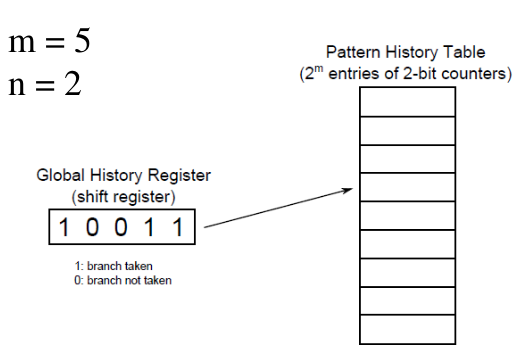
\includegraphics[scale=0.5]{immagini/corr_pred}
\subsection{Tournament predictor}
Si usano due tipi di predittori:
\begin{itemize}
\item correlated predictor, basato sugli ultimi m branches, acceduto dalla storia locale
\item local predictor, che viene selezionato usando l'indirizzo del branch
\end{itemize}
Si usa poi un indicatore di quale è stato il miglior predittore per lo specifico branch in esecuzione, che è un contatore a 2 bit, incrementato per uno dei predittori e decrementato per l'altro. Di seguito, uno schema dell'architettura del tournament predictor DEC Alpha 21264\\\\
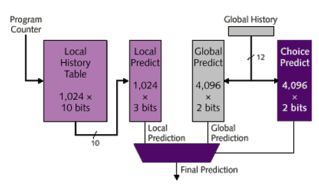
\includegraphics[scale=1]{immagini/tourn_pred}
\subsubsection{Branch target buffer}
È relazionato ai jump indiretti, che sono difficili da predirre. esempio: la ret è l'istruzione di ritorno da una sub routine. Il problema è capire dove si ritorna: qual è l'istruzione che si mette in pipeline, dovrebbe essere la prossima del chiamante ma è ancora più complicato. Si può fare il jump nell'indirizzo contenuto in un registro, l'output dipende da cosa è scritto nel registro che si vuole usare per il salto.\\ Il BTB è una picccola cache che viene acceduta col program counter 
%immagine dell'architettura
troviamo il prefetched target ed il prediction bit, che dice se conviene prendere il trarget oppure mettere uno stallo. È una cache, quindi ci può essere miss o hit, si può imparare se il prefetched target dovrebbe essere quello e più tardi si saprà se quel target è corretto o meno.
\subsubsection{Return address stack}
L'istruzione di ret legge l'indrizzo dallo stack, quindi se possiamo leggerlo subito possiamo sapere il target del ritorno.\\ Possiamo mettere uno stack nella CPU che manitene gli indirizzi di ritorno, ogni volta che c'è una chiamata, si salva in questo stack l'indirizzo di ritorno. In questo modo, ogni volta che si torna si conosce l'indirizzo di ritorno e questo è utilissimo perché l'85\% delle istruzioni è di ritorno.
\subsubsection{Fetch Both Target}
Tecnica che costa molto perché riempi la pipeline con tutte le istruzioni, ma la metà verranno scaratate e non aiuta in casi di fetch multipli come lo \textsf{switch}, non viene usato nell'hardware off the shelf.
%slides
\subsection{Simultaneus multi-threading}
C'è una CPU fisica ma è esposta al software come una coppia di CPU virtuali. L'idea è che mentre runni istruzioni nella pipeline usi un sotto-insieme delle risorse hardware, in questo caso nel simultaneous MT si puà tenere traccia di che hw stanno usando le istruzioni, quindi si duplica lo stato dell'architettura, quindi ad esempio il PC in modo che il processore usi un algoritmo di scheduling in modo da dare il controllo ai differenti thread che girano. Quindi è richiesto meno hw per far girare più processi ma servono dei controlli per evitare l'interferenza.
\subsubsection{Caso Intel: Hyperthreading}
Gli obiettivi sono molteplici:
\begin{itemize}
\item minimizzare la die area
\item evitare che uno dei due processori logici produca stalli per l'altro
\item "spegnere" l'hyperthreading se non necessario
\end{itemize}
Oggi, anche l'archiettura Inter mostra delle istruzioni assembly al programmatore diverse da quelle efeftivamente usate internamente, ci sono due parti:
\begin{itemize}
\item un front-end
\item un engine di esecuzione out-of-order: se puoi eseguire una micro operazione va eseguita immediatamente.
\end{itemize}
\paragraph{Xeon frontend:}il ruolo è quello di tradurre istruzioni CISC in istruzioni RISC usando una microcode ROM. C'è una cache di micro operazioni che mantiene le traduzione già fatte.\\ Nella trace cache, sappiamo se una micro operazione è associata ad uno o all'altro execution program, grazie ai due program counter differenti. Ci sono quindi due code diverse di micro operation. Nel caso di hit: %slides
\\ Nel caso di miss nella TC, serve fare la traduzione: bisogna accedere all'instruction TLB che permette di tradurre la corrispondenza fra indirizzi logici e fisici. Ovviamente, ci sono due TLB associati alla cache L2, quindi si può pagare anche un miss dovuto alla L2. Quindi, si mette la CISC instruction in coda, c'è poi il decoder ROM che mette le istruzioni in una coda usata per fillare la TC e quindi ora si può mettere la micro operation nella $\mu$op queue.
%slides
\paragraph{Xeon Out-of-order pipeline:}
%immagine
vogliamo eseguire le micro operazioni in ogni ordine quando è possibile farlo. Nel primo stadio, vogliamo schedulare i registri fisici della CPU: una $\mu$op cerca di accedere il registro icx, non è uno solo ma sono molteplici, i multi-registri e quindi icx viene mappato su uno di questi. Servono quindi un register rename ed un Allocate per tenere traccia di tutto.\\ Ora ci sono code multiple, per discriminare la semantica della $\mu$op in base al fatto che si acceda alla memoria etc...\\ Lo stadio di execute ha diverse ALU, quindi l'Allocation unit dice anche quale componente usare per eseguire l'istruzione. Lo scheduler prende l'istruzione dalla coda nel momento esatto in cui il componente è disponibile. L'ordine è qualsiasi, le $\mu$op appartengono a diversi program flow, quindi data una CISC operation, le macro istruzioni saranno invertite nell'ordine. \\ Alla fine, non vogliamo che le istruzioni siano materializzate all'esterno in ordine casuale, quindi c'è un reorder buffer per riordinare le istruzioni CISC nell'ordine in cui sono entrare e far credere all'utente siano state processate così.\\ Non abbiamo quindi una idea di come siano state eseguite le istruzioni internamente, quindi ci può essere uno stato di inconsitenza per un tempo illimitato ma non è un problema perché questo non viene esposto a livello ISA. Il problema è che stiamo interagendo con la memoria e questo è sfruttabile, possiamo ad esempio far si che la CPU carichi delle istruzioni che non doverebbe e quindi dei dati in cache che non dovrebbe: l'istruzione non verrà committata, ma la traccia sarà comunque esposta e sfruttabile.
\subsection{Multicores (2000s)}
I vendor cominiano ad usare i molteplici tansistor per creare delle CPU multicore, il primo CPU è l'IBM power4, 2 core con una architettura interessante: una cache privata per ciascun core, interconnessione di un certo tipo fra i core e una cache di L2 ed L3, dove la L3 fa anche da memory controller. I core interagiscono con la L1 e così a salire, quindi per caricare dati dalla memoria. Ma sei i cores hanno una cache privata, come fanno ad essere sincronizzati con i dati contenuti in L1 e quindi visibili al core 2? Serve un protocollo apposito per garantire la consistenza dei dati.
\subsubsection{Cache coherence}
Comportamento della cache da un punto di vista di utilizzo. La CC definisce la coerenza della cache con dei protocolli: quando scrivo codice, non mi rendo conto di interagire con la cache, ma i processori vi interagiscono di conitnuo. Abbiamo ad esempio 2 cores, con due cache private ed una serie di operazioni:
%carica la tabellina
al tempo 0, la cache del core 1 c'è la copia di A, a t=1 C2 carica A in un altro registro. Poi C1 fa una una operazione su A, quindi il valore di A nella cache di C2 quale sarà? Non c'è una sola risposta, dipenderà dal protocollo di consistenza
\paragraph{Strong CC protol:}il protocollo più semplice, tutte le cache dei vedono gli stessi dati, come se non ci fosse una separazione fra le cache in un qualunque istante di tempo. Quindi, serve avere un agreement fra i cores su chi fa l'operazione sul dato, quindi c'è un impatto sulla concorrenza e le perfomance.\\ Per assicurare tale consitenza serve:
\begin{itemize}
\item single write/multiple readers: ad ogni istante di tempo, per ogni locazione di memoria un solo core può leggere e scrivere
\item (slides)
\end{itemize}
Bisogna continuamente sincronizzare le cache quando un core fa un update in memoria, quindi non è molto performante
\paragraph{Coerenza debole:} c'è meno limitazione sulle cache, in quanto devono sincronizzarsi meno, quindi viene persa una delle invarianti dette sopra. Quindi due cores possono scrivere su una stessa area di memoria, quindi può accadere che il programmatore osservi dei comportamenti inattesi e quindi per implementare correttamente l'algoritmo occorre implementare delle primitive software per avere lo stesso outcome che si avrebbe se tutto accadesse sequenzialmente.\\ C'è una time window di un certo numero di epoche temporali in cui i dati non vengono propagati e questo può mostrare la complessità dell'hardware al programmatore\\\\ È anche possibile non avere coerenza, che è il modo per avere le cache più veloci. Non ci sono ovviamente garanzie, quindi le cache vanno sincronizzate esplicitamente lato software, ad esempio con delle API C/Assembly.
\subsubsection{CC protocol}
Un protocollo di consitenza per la cache è un algoritmo distribuito basato su primitive di tipo message-passing. Ci sono due principali tipi di richieste in memoria da servire:
\begin{itemize}
\item Load(A)
\item Store(A)
\end{itemize}
e coinvolge 2 tipi di attori principali, ovvero i cache controllers ed i memory controllers. Il ruolo è quello di rinforzare una certa nozione di coerenza.\\ Qualunque cosa nei protocolli CC è basato sulle coherency transaction, ciascuna di queste genere dei messaggi. Ci sono due tipi principali di transazioni:
\begin{itemize}
\item Get: carica un blocco di cache (dato) in una linea di cache
\item Put: evince un blocco dalla linea di cache, la linea diventa disponbile per altri dati
\end{itemize}
%immagine dell'organizzazione
Ogni linea di cache è associata con un bit che dice se la linea è valida o memo, in questo caso abbiamo una macchina a stati finiti che definisce lo stato del blocco in cache. La macchina è leggermente più complessa di una classi FSM, perché per transitare dai vari stati ci possono essere dei delay dovuti al fatto che il protocollo è distribuito. Ci sono quindi
\begin{itemize}
\item eventi remoti: viene ricevuto un messaggio di coerenza
\item eventi locali, ricevuti dalla parent cache
\end{itemize}
(altro sulle slides)\\ Ci sono una serie di protocolli per gestire la coerenza, definiamo
\begin{itemize}
\item invalidate protocols: protocolli, quando viene scritto un blocco invalida tutte le altre copie.
\item update protocols: ogni update viene mandato a tutti i core.
\end{itemize}
Quindi, nell'esempio iniziale il valore di A dipende dal protocollo implementato. Ci sono poi due famiglie di CC protcolos diversi
\begin{itemize}
\item snooping protocols: tutti i controller osservano tutto il traffico, quindi il broadcast è totalmente ordinato. È molto veloce, perché tutti i controller possono fare decisioni da soli perché osservano tutti i messaggi ma non è scalabile se il numero di core aumenta. Questo perché serve una arbitro del bus, e questo degrada le performance
%immagine snooping
\item directory based: c'è una directory, ogni request è unicast alla directory. Questa tiene traccia di chi è il controller destinatario e gli manda il messaggio, il che rende tutto più scalabile e permette di aumentare il numero di cores.
%immagine directory based
\end{itemize}
\subsubsection{VI protocol}
Il protocollo di consitenza più semplice, un solo cache controller può leggere e/o scrivere il blocco in ogni timestamp.\\ La transaction Get è usata per richiedere un blocco in read-mode per poter diventarne l'owner e potervi scrivere e leggere. La Put è usata per togliere il blocco dalla cache e riscriverlo al LLC controller. Ci sono una serie di eventi:
%copia slides
Il protocollo VI sta per Valid/Invalid, ma oltre a questi due stati ce n'è anche uno intermedio per cui si aspetta una copia del dato up-to-date
%immagine del FSM
Se confrontata con la FSM del LLC, vediamo che c'è differenza: ad un certo punto, il core associato al cache controller fa una operazione di load, quindi ottiene l'indirizzo e va nella cache e scopre che lo stato della cache è I. Quindi, serve una Own-Get dal LCC, manda un messaggio che viene ricevuto da tutti i cache controller nel sistema con un ordinamento totale. Una volta che il messaggio viene mandato, il controller trainsita nello stato IV, la copia verrà inviata dal possessore attuale del dato, dopo averlo ricevuto transita in V. \\ Dopo, un altro core vorrà diventare l'owner e quindi questo controller transiterà nello stato I e trasferirà il contenuto del blocco.\\ Immaginiamo di essere in una situazione in cui c'è un conflitto, ovvero si vuole scrivere un blocco nella linea di cache che è piena. Si manda una Any Put al LLC controller, l'LLC transita nello stato I e se poi qualcuno richiede il dato transita nello stato V.\\ Il protocollo ha una nozione implicita di diryness: se una linea di cache è in stato V, il controller L1 può o leggere e scrivere o solo leggere. Ha anche un concetto implicito di esclusività, in quanto se lo stato è V, nessun altro può accedere al blocco, quindi nessuno ha una copia valida; inoltre, c'è nozione del possesso del blocco: l'owner sarà quello che manda la copia aggiornata a tutti.\\ La cosa positiva del portocollo è che richiede pochi bits per rappresentare le FSM, ma ha diverse inefficienze; ciò che vogliamo catturare del blocco di cache sono aspetti di
\begin{itemize}
\item validità
\item dirtyness
\item exclusivity
\item ownership
\end{itemize}
vogliamo solo queste proprietà per avere un protocollo efficiente ma che consumi più bits per l'implementazione
\subsubsection{MOEST stable states}
Ogni lettera fa riferimento ad uno stato particolare, ognuno cattura una delle proprità dette sopra. Di nuovo, è una FSM per ogni blocco
\begin{itemize}
\item Modified: il blocco è valido, esclusivo, posseduto e potenzialmente dirty.Può essere scritto o letto
\item Owned: blocco valido, posseduto 
\item Shared: valido, non esclusivo, non posseduto, non sporco. Ci sono più copie read only del blocco.
\end{itemize}
(slides)\\ Quali sono le transazioni per poter implementare il protocollo:
\begin{itemize}
\item GetS: Get del blocco in Shared state
\item GetM: Get in modo Modified
\item Upgr: ho un blocco, so che il blocco ha la copia più aggiornata perché ho osservato le transazioni, quindi non voglio la copia del dato ma voglio la possibilità di scrivervi
\item Put (slides)
\end{itemize}
Questa è la macchina a stati che si ha tipicamente: 
%immagine della macchina
\subsubsection{MEST protocol}
Il controller della cache di livello inferiore (LLC) è simile 
%immagine
M/E è uno stato congiunto di Modified/Exclusive. Se in M/E e si osserva una Any-Get, si va in Shared, se qualcuno richiede il blocco, si va in I.
\subsection{Memory Control}
Nelle cache write through, si propaga direttamente l'update.\\ In modern architectures, the cache are no longer write through, due to the complexity can explode.\\ The caches in modern architectures can be either inclusives or exclusives at different levels, this can be exploited by attacks that specifically targets a L* cache.\\ CC dicatates how the different cache controllers interacts among them. There is the concept of memory consistence: il MC model definsce il comportamentio di una memoria condivisa, indipendentemente da come è implementata. Vediamo ancora un esempio:
%tabella esempio
in macchine Multi Core c'è il riordino degli accessi in memoria: il core committa le operazioni sulla memoria in un certo ordine ma gli altri cores possono osservarle in ordine diverso, quindi non c'è un ordinamento totale. Il sotto-sistema può quindi riordinare le operazioni: 
%tabella di esempio
ci sono 4 combinazioni di possibili riordini, quindi se scriviamo codice concorrente, dobbiamo considerare il fatto che ci siano riordini delle operazioni.\\ Questo ha a che fare con due ordinamenti diversi:
\begin{itemize}
\item ordiamento di programma, è per core ed è totale. Cattura l'ordine in cui ogni core 
\item ordinamento di memoria (slides)
\end{itemize}
Possiamo avere diverse consistenze:
\begin{itemize}
\item sequenziale: ci sono determiante operazioni che verranno osservate identicamente tra ordine di programma ed ordine di memoria.\\ Nell'esempio di prima, solo due ordini sono consitenti sequenzialmente
\item consitenza debole: modello implementato dalle architetture moderne. Quella di Intel è Total Order Store. C'è un piccolo buffer che agisce come coda in cui vengono salvate le diverse operazioni di store e che verranno poi processate. Le architetture Intel sono fra quelle in cui c'è il minimo numero di riordini tra le operazioni
\end{itemize}
\subsubsection{Memory fence}
Se ho una qualunque operazioni di memoria, la fence forza l'ordine di una load/store, quindi possiamo creare dei punti in cui siamo sicuri che tutte le istruzioni prima della fence sarà ordinata e stessa cosa se accade prima, ma non si possono riordinare le fence. Sono quindi operazioni speciali che permettono di mettere dei punti di riordino per poter ad esempio avere consitenza sequenziale in Intel.
\paragraph{Fence su architetture x86:} ci sono 3 tipi di fence diverse su x86:
\begin{itemize}
\item MFENCE: barriera full memory, ogni operazione prima e dopo non sarà riordinata
\item SFENCE: barriera store/store
\item LFENCE: barriere load/load e Load/Store
\end{itemize}
\section{In memory transaction}
Una transazione in memory permettono di realizzare la sincronizzazione in memoria più semplice. Può essere esplicita, quindi per accedere ad un sezione critica si prende un lock, si accede e poi si esce.\\ Ci possono essere problemi sui locks come deadlock, i deadlocks non sono componibili e quindi possono esserci delle inconsitenze nei risultati di operazioni che usano i lock.\\ L'hardware transactional Memory prevede di usare delle istruzioni di Assembly specifiche per dire che su vuole accedere a dei dati in maniera esclusiva, così che il processore metta un lock privato sui dati e una volta finito, se il commit va a buon fine i dati vengano pubblicati all'esterno\\ Per poter implementare le hw transaction Intel ha modificato il protocollo di CC: i tentativi vengono fatti solo al primo livello della cache e si marcano i blocchi di cache con lock, per poi committare se va tutto bene. Ci sono 4 nuove istruzioni assembly (slides), esempio in C:
% codice del C ed Assembly
Una transazione può andare in abort per vari motivi (slides)\\ Da un punto di vista di performance il problema è per cosa di fa abort a livello hardware, ma la cosa interessante è che la transazione può essere mandata in abort da qualunque altro CPU core.
\end{document}